\renewcommand*{\arraystretch}{1.1}

\noindent\begin{tabularx}{17cm}{|>{\small \sf}c|X|}
	\hline
	query    & BI / 22 \\ \hline
%
	title       & International dialog \\ \hline
%
    pattern     & \hfill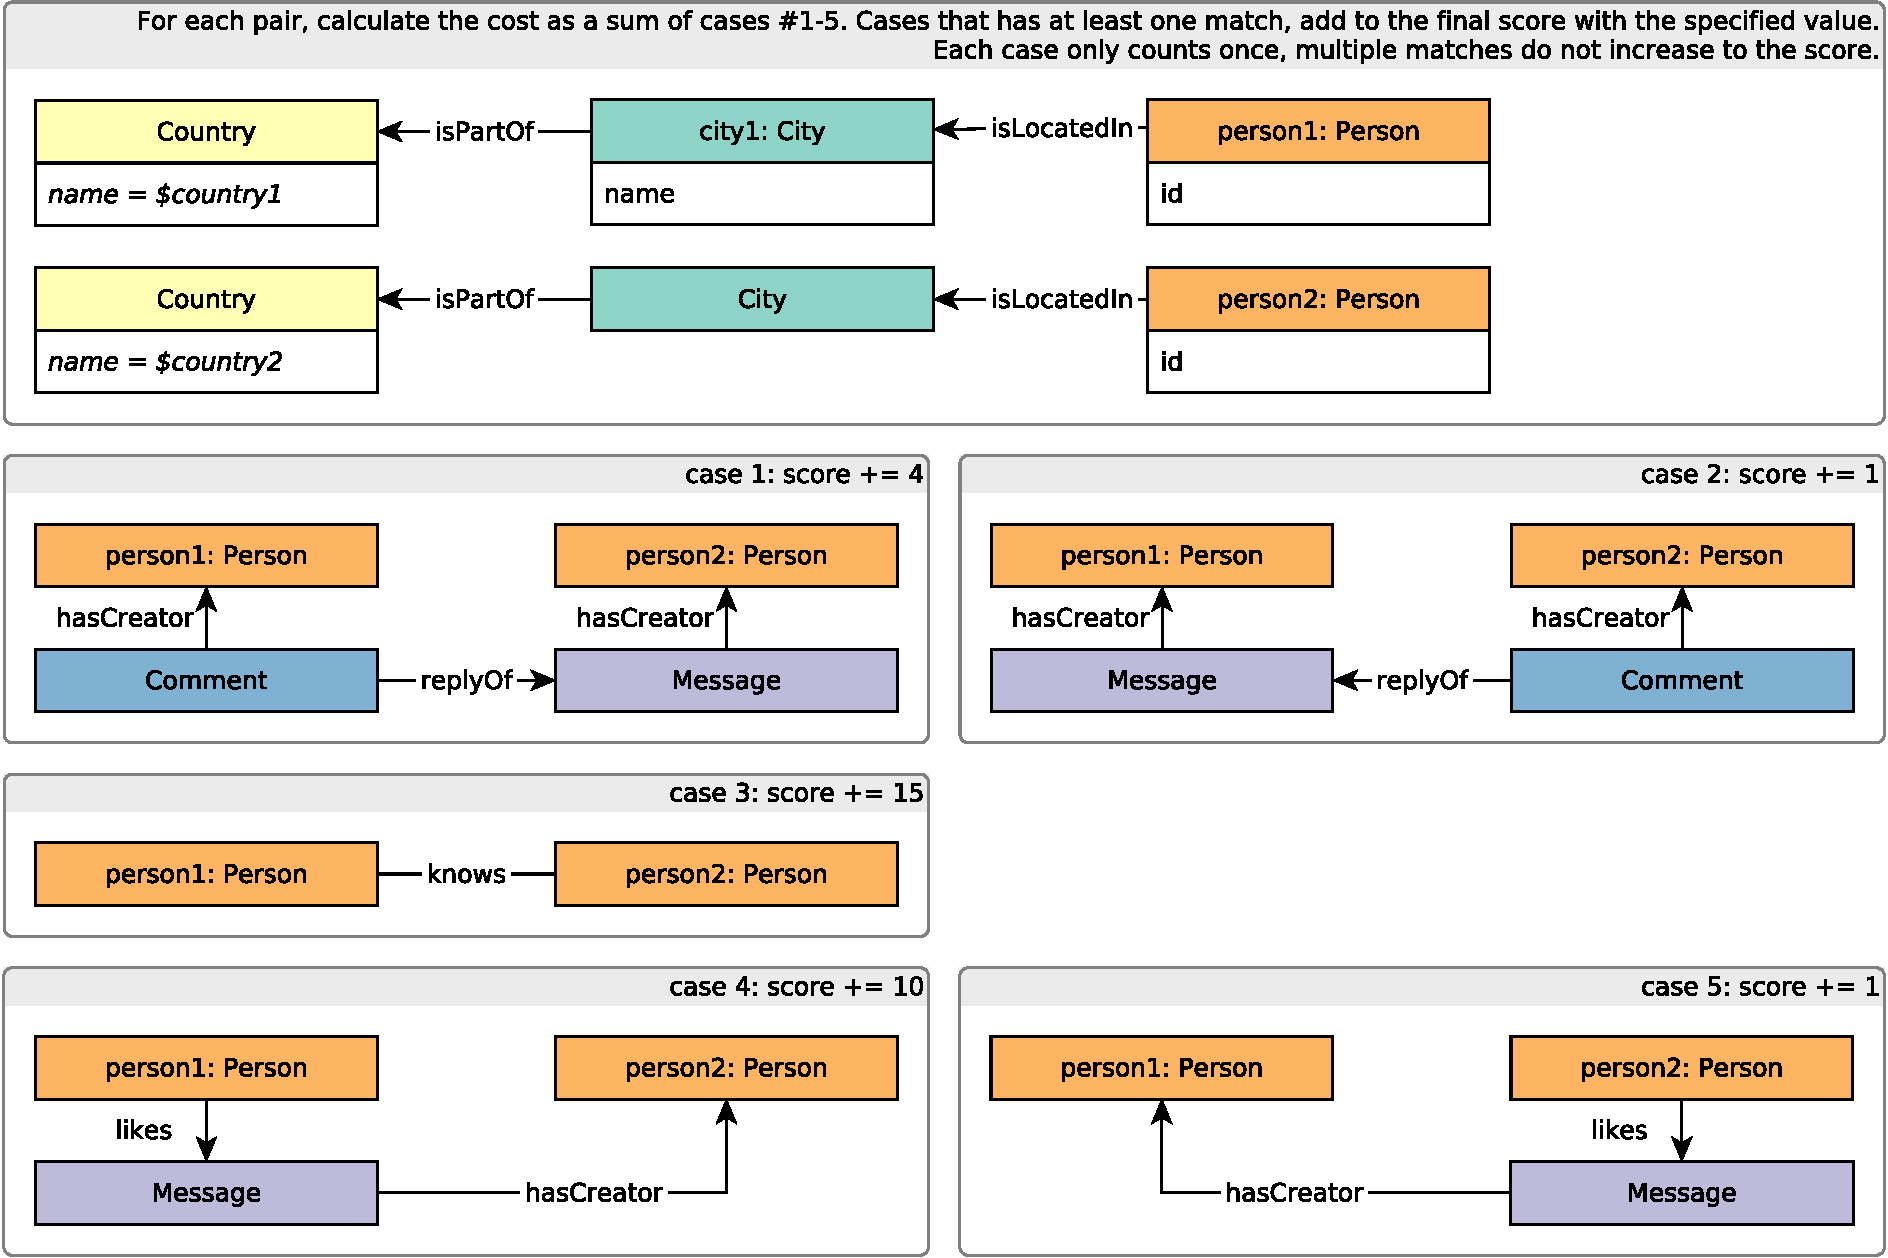
\includegraphics[scale=\patternscale,margin=0cm .2cm]{patterns/bi-read-22}\hfill\vadjust{} \\ \hline
%
	desc. & Consider all pairs of people \texttt{(p1,\ p2)} such that one is located
in a city of Country \texttt{countryX} and the other is located in a
city of Country \texttt{countryY}.

For each city of Country \texttt{countryX}, return the highest scoring
pair.

The score of a pair is defined as the sum of the scores of the following
kinds of interaction:

\begin{itemize}
\tightlist
\item
  \texttt{p1} has created a reply Comment to at least one Comment or
  Post by \texttt{p2}: \texttt{Score\ =\ 4}
\item
  \texttt{p1} has created at least one Post or Comment that \texttt{p2}
  has created a reply Comment to: \texttt{Score\ =\ 1}
\item
  \texttt{p1} and \texttt{p2} Know each other: \texttt{Score\ =\ 15}
\item
  \texttt{p1} liked at least one Post or Comment by \texttt{p2}:
  \texttt{Score\ =\ 10}
\item
  \texttt{p1} has created at least one Post or Comment that was liked by
  \texttt{p2}: \texttt{Score\ =\ 1}
\end{itemize}

I.e., the maximum score a pair can obtain is:
\texttt{4\ +\ 1\ +\ 15\ +\ 10\ +\ 1\ =\ 31}
 \\ \hline
%
	
%
	params.  &
	\vspace{1.1ex}{\begin{tabularx}{14.2cm}{|c|M|m{2cm}|Y|} \hline
	\cellcolor{parameter} \color{white} $\mathsf{1}$ & \varname{countryX} & \cellcolor{gray!20} \vartype{String} &  \\ \hline
	\cellcolor{parameter} \color{white} $\mathsf{2}$ & \varname{countryY} & \cellcolor{gray!20} \vartype{String} &  \\ \hline
	\end{tabularx}}\vspace{1.1ex} \\ \hline
%
	
	result      &
	\vspace{1.1ex}{\begin{tabularx}{14.2cm}{|c|M|m{2cm}|c|Y|} \hline
	\cellcolor{result} \color{white} $\mathsf{1}$ & \varname{p1.id} & \cellcolor{gray!20} \vartype{64-bit Integer} &
	    \texttt{R} &
	     \\ \hline
	\cellcolor{result} \color{white} $\mathsf{2}$ & \varname{p2.id} & \cellcolor{gray!20} \vartype{64-bit Integer} &
	    \texttt{R} &
	     \\ \hline
	\cellcolor{result} \color{white} $\mathsf{3}$ & \varname{cityX.name} & \cellcolor{gray!20} \vartype{String} &
	    \texttt{R} &
	     \\ \hline
	\cellcolor{result} \color{white} $\mathsf{4}$ & \varname{score} & \cellcolor{gray!20} \vartype{32-bit Integer} &
	    \texttt{C} &
	     \\ \hline
	\end{tabularx}}\vspace{1.1ex} \\ \hline
	
%
	sort        &
	\vspace{1.1ex}{\begin{tabular}{|c|l|c|} \hline
	\cellcolor{sort} \color{white} $\mathsf{1}$ & \varname{score} & \cellcolor{gray!20} $\desc$ \\ \hline
	\cellcolor{sort} \color{white} $\mathsf{2}$ & \varname{p1.id} & \cellcolor{gray!20} $\asc$ \\ \hline
	\cellcolor{sort} \color{white} $\mathsf{3}$ & \varname{p2.id} & \cellcolor{gray!20} $\asc$ \\ \hline
	\end{tabular}}\vspace{1.1ex} \\ \hline
	%
	%
	CPs &
	\multicolumn{1}{>{\raggedright}l|}{
	  \chokepoint{1.4}, 
	  \chokepoint{1.6}, 
	  \chokepoint{2.1}, 
	  \chokepoint{3.1}, 
	  \chokepoint{3.3}, 
	  \chokepoint{5.1}, 
	  \chokepoint{5.2}, 
	  \chokepoint{5.3}
	  } \\ \hline
	%
    %
\end{tabularx}
\vspace{2ex}